\documentclass[tikz,border=5mm]{standalone}
\usetikzlibrary{calc,intersections}
\usetikzlibrary{patterns}
\begin{document}
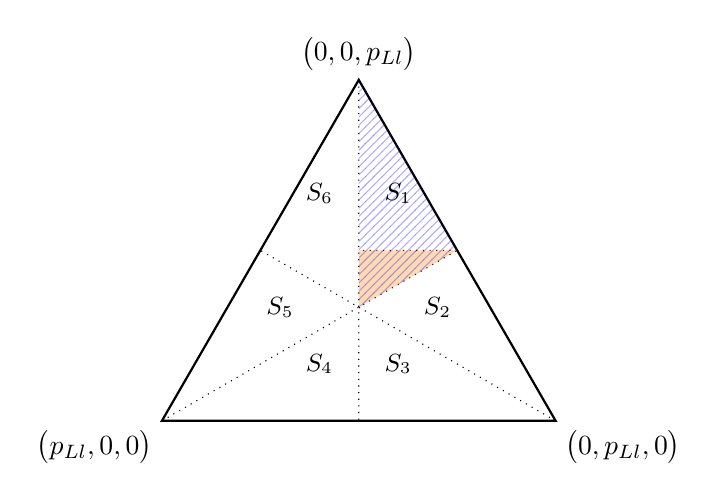
\begin{tikzpicture}[scale=5]
	% Define vertices
	\coordinate (A) at (0,0);
	\coordinate (B) at (1,0);
	\coordinate (C) at (0.5,0.866);
	
	% Draw triangle
	\draw[thick] (A) -- (B) -- (C) -- cycle;
	
	% Vertex labels
	\node[below left]  at (A) {$\bigl(p_{Ll},0,0\bigr)$};
	\node[below right] at (B) {$\bigl(0,p_{Ll},0\bigr)$};
	\node[above]       at (C) {$\bigl(0,0,p_{Ll}\bigr)$};
	
%	\node[below left, xshift=-0.02cm, yshift=0.4cm]  at (A) {$p_{Hh}$};
%	\node[below right, xshift=0.02cm, yshift=0.4cm] at (B) {$p_{Hl}$};
%	\node[above, xshift=0.4cm, yshift=-0.2cm]       at (C) {$p_{Lh}$};
	
	% Midpoints of edges
	\coordinate (MAB) at ($ (A)!0.5!(B) $);
	\coordinate (MBC) at ($ (B)!0.5!(C) $);
	\coordinate (MCA) at ($ (C)!0.5!(A) $);
	
	% Medians (dotted)
	\draw[dotted] (C) -- (MAB);
	\draw[dotted] (A) -- (MBC);
	\draw[dotted] (B) -- (MCA);

	
	% Intersection of medians (centroid)
	\path[name path=median1] (C) -- (MAB);
	\path[name path=median2] (A) -- (MBC);
	\path [name intersections={of=median1 and median2, by=G}];
	
	\path[name path=horizontalcut] (MBC) -- (MCA);
	
	% Define path of A -- MAB
	\path[name path=medianA] (C) -- (MAB);
	
	% Compute intersection
	\path [name intersections={of=horizontalcut and medianA, by=I}];
	
	% Draw the horizontal cut only up to the intersection
	\draw[dotted] (MBC) -- (I);
	
	\fill[orange, opacity=0.3] (MBC) -- (I) -- (G) -- cycle;
	    \begin{scope}[opacity=0.3] % adjust opacity here (0 = fully transparent, 1 = fully opaque)
		\fill[pattern=north east lines, pattern color=blue] (C) -- (G) -- (MBC) -- cycle;
	\end{scope}
%	
%	% Mark centroid
%	\filldraw[red] (G) circle (0.5pt) node[below right] {$G$};
%	
	% Label regions
	% S1 in top right region (around G, C, MAB)
	\node at ($ (G)!0.6!(C) + 0.4*(MAB) - 0.2*(G) $) [font=\small] {$S_1$};

	% S2 in bottom right region (G, B, MBC)
	\node at ($ (G)!0.2!(B) + 0.2*(MBC) - 0.1*(G) $) [font=\small] {$S_2$};

	% S3 in bottom region (G, MBC, MAB)
	\node at ($ (G)!0.8!(MBC) + 0.7*(MAB) - .9*(G) $) [font=\small] {$S_3$};

	% S4 in bottom left region (G, A, MAB)
	\node at ($ (G)!0.3!(A) + 0.3*(MAB) - 0.2*(G) $) [font=\small] {$S_4$};

	% S5 in top left region (G, A, MCA)
	\node at ($ (G)!0.2!(A) + 0.4*(MCA) - 0.4*(G) $) [font=\small] {$S_5$};

	% S6 in top region (G, C, MCA)
	\node at ($ (G)!0.6!(C) + 0*(MCA) - 0.2*(G) $) [font=\small] {$S_6$};

	
\end{tikzpicture}


\end{document}